\documentclass[tikz, border=10pt]{standalone}
\usetikzlibrary{arrows.meta, positioning}

\begin{document}
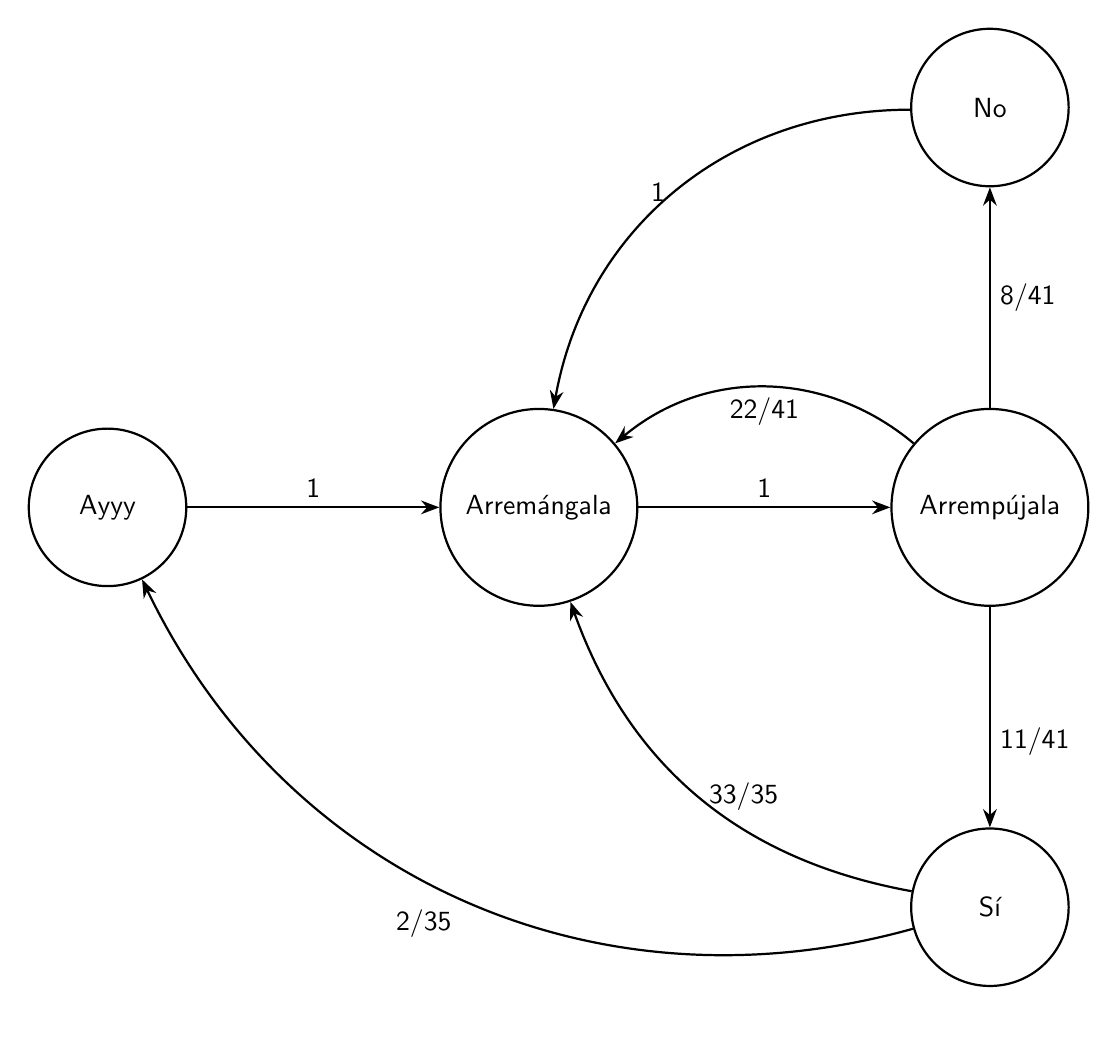
\begin{tikzpicture}[
  node distance=2.8cm and 3.2cm,
  every node/.style={font=\sffamily},
  state/.style={circle, draw, minimum size=20mm},
  bigstate/.style={circle, draw, minimum size=25mm},
  every path/.style={->, thick, >=Stealth}
]

% Nodes
\node[state] (ayyy) {Ayyy};
\node[bigstate, right=of ayyy] (arremangala) {Arremángala};
\node[bigstate, right=of arremangala] (arrempujala) {Arrempújala};
\node[state, below=of arrempujala] (si) {Sí};
\node[state, above=of arrempujala] (no) {No};

% Arrows
\draw (ayyy) -- node[above] {1} (arremangala);
\draw (arremangala) -- node[above] {1} (arrempujala);
\draw (arrempujala) -- node[right] {8/41} (no);
\draw (arrempujala) -- node[below right] {11/41} (si);
\draw (arrempujala) to[bend right=40] node[below] {22/41} (arremangala);
\draw (no) to[bend right=40] node[left] {1} (arremangala);
\draw (si) to[bend left=30] node[right] {33/35} (arremangala);
\draw (si) to[bend left=40] node[below left] {2/35} (ayyy);

\end{tikzpicture}
\end{document}
